\chapter{Introduction}
\label{sec:introduction}

\subsection{Motivation}
\label{sec:motivation}

% \todo[inline]{lots of ``systems'' written here}

Modern physical systems, particularly those associated with public use such as freeway networks and water supplies, exist within a world with decreasing physical space and resources. For instance, freeways often cannot add additional lanes to accommodate increased demands. Thus, one must rely upon better management systems and control algorithms in order to maximize performance within the limitations of the existing system. These ``smart'' systems make use of sensing instrumentation to estimate real-time conditions and modeling of the underlying physical dynamics to predict and plan for future states.

The focus of this thesis is the development of methods for the intelligent modeling and control of such networked dynamical systems. The goal is to provide operational managers with scalable, flexible, and robust algorithms that can leverage the well-instrumented and highly-connected control infrastructure present on modern systems. 

The remainder of this section discusses the \emph{Connected Corridors} project (Section~\ref{sec:connected-corridors}) on integrated freeway-corridor management (ICM), which served as the context in which this work was conducted, followed by an overview of \emph{model predictive control} (MPC) methods and their suitability in solving some of the main objectives put forth in the \emph{Connected Corridors} project (Section~\ref{sec:model-predictive-control}). The section concludes with a summary of the original contributions presented in this thesis (Section~\ref{sec:contributions}).

\subsection{Connected Corridors}
\label{sec:connected-corridors}

\emph{Connected-Corridors} is a project funded by the California Department of Transportation with the goal of creating the next generation of traffic management tools~\cite{connected-corridors,miller2010san}. While most current systems consider the freeway networks as independent from the city-street \emph{arterial} road networks, \emph{Connected Corridors} is tasked with creating an integrated approach to traffic management (referred to as ICM) which accounts for their dual performance. The project has demonstrated innovative control and estimation approaches to ICM on macroscopic and microscopic simulation environments (presented in Section~\ref{sec:numerical-results-adjoint}), with the ultimate plan of transferring the knowledge to a physical test-site within California.

The proposed ICM system possesses the following capabilities.

\begin{itemize}
	\item \textbf{Estimation}: Operators have access to a real-time estimation of the traffic conditions along the major freeways and adjacent arterials~\cite{work2010traffic,Jacqueta}.
	\item \textbf{Simulation}: Well-calibrated and efficient traffic models allow operators to simulate many different future traffic conditions~\cite{Muralidharan2009b,dervisoglu2014macroscopic}.
	\item \textbf{Control}: Traffic signal and message sign plans are computed online for many specialized objectives and serve as an optimized decision support tool~\cite{Reilly2013b,Reilly2014b}.
\end{itemize}

Control schemes implemented by the system include coordinated traffic light metering plans on freeway onramps (commonly referred as ramp metering, see Section~\ref{sec:continous-and-discrete-traffic-model-for-ramp-metering}) and traffic flow diversion around incidents via changeable message signs~\cite{Samaranayake2014}. 

\begin{figure}[htbp]
	\centering
	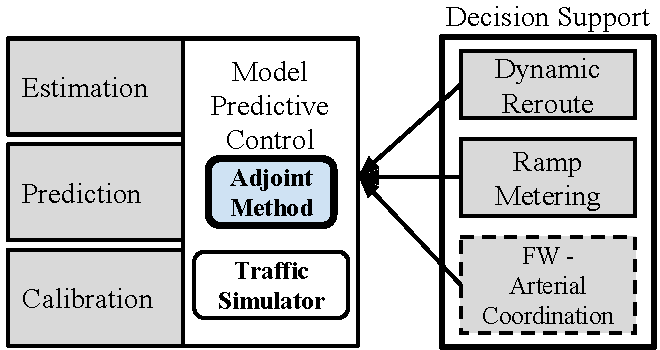
\includegraphics[width=0.8\textwidth]{diagrams/f2}
	\caption{\emph{Connected Corridors} control system architecture. The freeway state estimation, prediction and calibration submodules enable an MPC-based framework that computes coordinated, predictive decision-support strategies for numerous applications. Limited customization is required to extend the adjoint-based MPC controller to specific objectives or actuation types.}
	\label{fig:decision-support}
\end{figure}

To satisfy the above requirements, \emph{Connected Corridors} focuses on a number of submodules which are developed independently, but composed arbitrarily to create high-level, comprehensive support tools. Figure~\ref{fig:decision-support} shows a diagram of the several of the developed submodules and how they can be composed to create an MPC controller (explained in Section~\ref{sec:model-predictive-control}). Subsequently, the controller submodule is leveraged by a number of actuation strategies which have similar architectural requirements. For instance, both ramp metering and dynamic rerouting require real-time estimation and a calibrated freeway model to compute effective control strategies. Via submodule composition, much of the technology can be reused between the applications. This work contains the theory and implementation of constructing such controller submodules which efficiently exploit the structure of freeway networks.

\subsection{Model Predictive Control}
\label{sec:model-predictive-control}

Central to the \emph{Connected Corridors} approach of freeway traffic decision support is the concept of \emph{model predictive control} (MPC)~\cite{Muralidharana,o2013splitting,Frejo2011}. Generally speaking, MPC schemes successively compute a control policy which maximizes the performance, according to a provided criteria, of the system over the immediate future, where this work assumes the future to be of finite duration. The policy generated from the MPC scheme is recomputed as frequently as the real-time state estimation and computation times permit. Thus, associated with an MPC problem are two time periods: the \emph{update time} representing how often the MPC policy is recomputed online, and the \emph{time horizon} representing how far into the future for which the MPC policy will account. A more detailed treatment of MPC schemes is given in Section~\ref{sec:model-predictive-control-overview-adjoint-section}.

The requirements of an online MPC controller for a traffic system are depicted in Figure~\ref{fig:decision-support}. At the base of the method is a mathematical model of the physical system, referred to as the \emph{forward system}. These models often require calibration using historical sensor measurements to set the model parameters. To fully specify the simulation, an \emph{initial condition} is specified (i.e. estimation), as well as the \emph{boundary conditions} at the exteriors of the system over the entire time horizon of the MPC problem (i.e. prediction). All these requirements are satisfied by components within the \emph{Connected Corridors} system~\cite{Muralidharan2009b,dervisoglu2014macroscopic,work2010traffic}, making MPC control a natural fit for research and development in the project.

The focus of this thesis is the efficient and flexible design of MPC optimization techniques and their applications to freeway control systems. At the heart of the developed approach is the \emph{discrete adjoint} method for gradient computations within first-order gradient descent methods (Section~\ref{chapter:adjoint}). The efficiency of the developed method enables \emph{online} application of MPC to the control of large freeway networks (on the order of tens of miles) with frequent recomputations (on the order of one minute) to ``close the loop'' with real-time measurements.

In addition to the well-established ramp metering control infrastructure, the emergence of smartphones and connected vehicles has made mass rerouting strategies a new, viable form of control. This thesis acknowledges this potential by including an investigation of rerouting strategies for a subset of flow on networks. Inspired by the increasing penetration navigation devices in vehicles (e.g. dedicated units, smartphone applications), a single navigation provider may advise a signification portion of the total flow on some networks, thus potentially affecting traffic conditions based on their advice. This potential can be harnessed to reduce the inefficiencies of \emph{selfish routing}~\cite{Krichene2012c,Roughgarden2002How} and drive network behavior towards \emph{socially optimal} conditions.

\subsection{Contributions}
\label{sec:contributions}

This thesis contains the following contributions to the problem of optimal control of networked dynamical systems.

\begin{itemize}
	\item \textbf{A novel continuous freeway traffic model suitable for finite-horizon optimal control problems}~\cite{delle2014pde,Reilly2013b}.
	\begin{itemize}
		\item The model represents an extension of the networked \emph{Lighthill-Richards-Whitham} (LWR) PDE traffic model~\cite{lighthill1955kinematic,richards1956shock} proposed in~\cite{garavello2006traffic}, where onramps are modeled as ODE buffers to guarantee \emph{strong} boundary conditions and flow conservation at the network boundaries.
		\item A discretized version of the continuous model is derived for optimal control application using Godunov's method~\cite{godunov1959,lebacque1996godunov}.
	\end{itemize}
	\item \textbf{A method for optimal control of networked conservation law systems based on discrete adjoint calculations}~\cite{Reilly2013b,Samaranayake2014}.
	\begin{itemize}
		\item This work develops a framework for converting a continuous time and space control problem on a physical network, where edges behave according to a conservation law, into a discrete, finite-horizon optimal control problem using Godunov discretization.
		\item The application of the discrete adjoint method~\cite{Giles2000,Duffy2009,d2010modeling,Gugat2005} to compute gradients for the above problem is presented, with an analysis of the linear scalability of the approach in discrete time and discrete space for sparse network structures.
		\item An explicit formulation of the discrete adjoint method is given for the application of coordinated ramp metering control~\cite{Papageorgiou1991,Frejo2011,Kotsialos2004,gomes2006optimal} for freeway networks.
		\item MPC numerical simulations on a macroscopic model of the I15 South Freeway in San Diego, California demonstrate the practical nature and the robustness to measurement noise of the research.
	\end{itemize}
	\item \textbf{A decentralized algorithm and control infrastructure for networked dynamical systems}~\cite{Reilly2014b}.
	\begin{itemize}
		\item This thesis presents a new distributed optimization method based on the alternating directions methods of multipliers (ADMM)~\cite{Boyd2010a,gabay1976dual,mota2012distributed} algorithm for solving  optimal control problems over subnetworks in parallel. The splitting method is done in such a way to only require communication between physically-neighboring subnetworks.
		\item Differing from similar work where subsystems only share control variables~\cite{mota2012distributed,camponogara2009distributed}, the presented method allows for subsystems to share both control \emph{and state} variables, an assumption necessary for the distributed control of traffic networks and hydrological systems.
		\item A discrete adjoint formulation is presented for efficient solution of subsystems with coupled control and state variables.
	\end{itemize}
	\item \textbf{An analysis of the security of traffic control systems and coordinated ramp metering attacks}~\cite{Reilly2014c,Reilly2014a}.
	\begin{itemize}
		\item A classification of traffic system vulnerability locations is constructed across such categories as cost of attack, effectiveness, and directness of control.
		\item A novel analysis of the potential damage and impact of coordinated ramp metering attacks is conducted using adjoint-based optimal control and multi-objective optimization tools.
		\item Illustrative attack scenarios are constructed and numerically investigated on realistic freeway networks. A web-based coordinated ramp metering attack tool was created to implement the interactive optimization approaches presented in the work~\cite{smartroadswebsite}.
	\end{itemize}
	\item \textbf{A framework for rerouting a subset of vehicles on freeway networks}.
	\begin{itemize}
		\item As opposed to standard system-optimal routing problems~\cite{ziliaskopoulos2000linear,Kelly} where all flow is controllable, we construct a network-flow optimization problem which allows one to specify a \emph{compliance rate} of cooperative vehicles. The proposed model captures the delays induced by the noncompliant vehicles.
		\item To account for the possibility of noncompliant drivers adapting to the new flow conditions, we propose a behavioral model, referred to as \emph{bounded tolerance}, which assumes that noncompliant drivers have bounded rationality and will only switch routes under significant increases in delay.
		\item Numerical examples for communication networks and freeway systems demonstrate the effectiveness of the method.  
	\end{itemize}
\end{itemize}

\subsection{Organization}
\label{sec:organization}

The rest of the article is organized as follows.

Chapter~\ref{chapter:freeway-network-model} presents the continuous and discrete freeway models which serves as the running application of the theory presented subsequently.  After covering preliminaries on networked PDE systems, the derivation of and motivation behind the model are given.

Chapter~\ref{chapter:adjoint} presents the discrete adjoint approach to optimal control of networked conservation laws. Presented first is a general overview of the discrete adjoint method, followed by its specific instantiation for discretized physical network systems. The application to coordinated ramp metering is then presented with numerical examples. The chapter concludes with the distributed, asynchronous formulation of the adjoint optimal control method via subnetwork splitting.

Chapter~\ref{chapter:security} presents a study of traffic control systems and their vulnerabilities. After defining the specific control system under consideration and its security weaknesses, the work gives an in-depth study of coordinated ramp metering attacks.

Finally, we conclude with a overview of the work presented, as well as directions for future research.